\documentclass[12pt,a4paper,openright]{mwrep}

\usepackage{lmodern}
\usepackage[T1]{polski}
\usepackage[utf8]{inputenc}

\usepackage[a4paper,
            tmargin=2cm,
            bmargin=2cm,
            lmargin=2cm,
            rmargin=2cm,
            bindingoffset=0cm]{geometry}

\usepackage{tocloft}
\usepackage{hyperref}

\usepackage{amsmath}
\usepackage{amssymb}
\usepackage{siunitx}

\usepackage{listings}

\usepackage{graphicx}
\usepackage{subfig}


\hypersetup{
    colorlinks,
    citecolor=black,
    filecolor=black,
    linkcolor=black,
    urlcolor=black
}

\newtheorem{definition}{Def}

\begin{document}

\title{%
Technika cyfrowa\\
Sprawozdanie 1\\
}

\author{\\Jan Chyczyński\\Błażej Nowicki
\\Bartłomiej Słupik\\Przemysław Węglik}

\date{\today}

\maketitle

\chapter{Zadanie 1a}

\section{Wstęp}
Zadanie polega na zaprojektowaniu układu realizującego 
funkcję logiczną:
\begin{align*}
    Y = \overline{A}C + B(A + B)
\end{align*}
Układ można zrealizować wyłącznie dzięki użyciu bramek NAND
ponieważ bramka NAND jest systemem funkcjonalnie pełnym tzn.
korzystając wyłącznie z niej można przedstawić dowolną funkcję
boolowską.



\section{Rozwiązanie teoretyczne}
Pierwszym krokiem jest przekształcenie wyrażenie do zawierającego
wyłączenie operacje NAND.
\begin{align*}
    Y &= \overline{A}C + B(A + B) \\
    &= \overline{\overline{\overline{A}C}\overline{B}}
\end{align*}

\section{Symulacja w programie Multisim}
Program został napisany w~języku~Python w wersji 3.8.
Do stworzenia aplikacji graficznej użyto
biblioteki~pygame\footnote{\url{https://www.pygame.org}}.

\section{Wnioski}
Celem implementacji struktur jest
stworzenie optymalnego
algorytmu odpowiadającego na zapytanie:



\chapter{Zadanie 1b}


Wykorzystamy funkcję działajacą w~następujący sposób:
    \begin{enumerate}
        \item porównanie obszaru zapytania z~aktualnie rozważanym wierzchołkiem,
        \begin{enumerate}
            \item jeśli obszar zawiera rozważany punkt, dodaj go do zbioru wynikowego,
        \end{enumerate}
        \item wywołaj funkcję rekurencyjnie dla każdego podobszaru przecinajacego się
        z~obszarem zapytania.
    \end{enumerate}
W~ten sposób w~każdym kroku zmniejszamy obszar poszukiwań.

Złożoność:
\begin{itemize}
    \item $O(\log n)$ dla pojedynczego punktu,
    \item $O(m\log n)$ dla zadanego obszaru, gdzie $m$ to ilość punktów w~tym obszarze.
\end{itemize}

Na Rys.~\ref{rys:example_picture} przedstawiono animację znajdującą pojedyczny punkt na płaszczyźnie
(sytuacja ta jest zatem tożsama ze wstawianiem punktu).
Jak widzimy podziały nie zawsze są równe.
Wynika to z~niezbalansowania drzewa.

\begin{figure}[h]
    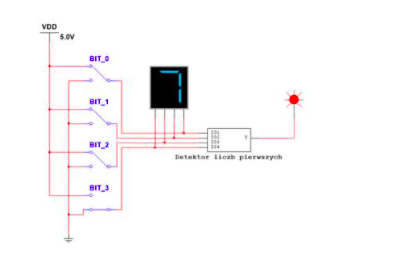
\includegraphics[width=0.44\textwidth]{images/example.png}
    \caption{Wyszukiwanie pojedynczego punktu w drzewie czwórkowym}
    \label{rys:example_picture}
\end{figure}

\end{document}
